% !TeX root = ../main.tex
% Add the above to each chapter to make compiling the PDF easier in some editors.
\chapter{Data Usage Screenshots}
\begin{center}
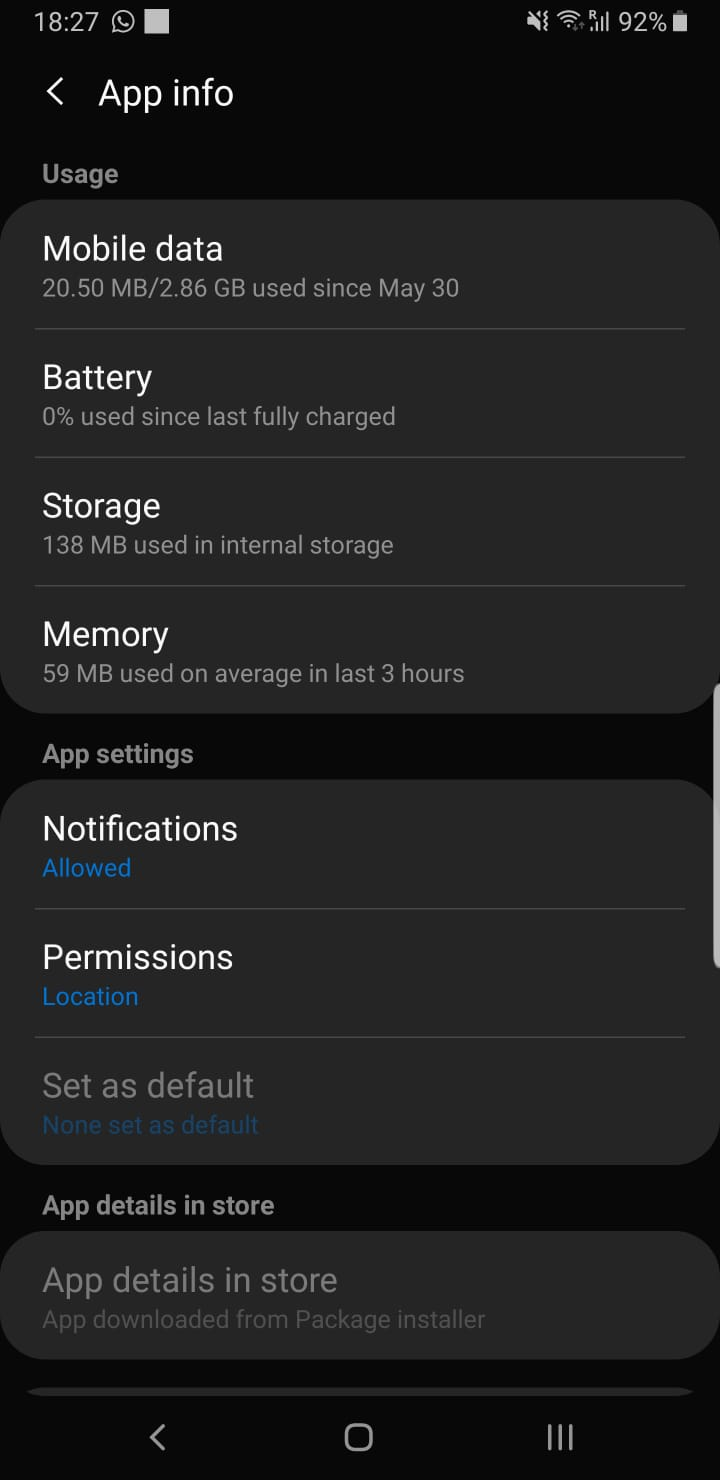
\includegraphics[width=0.5\textwidth]{data/data-usage/data-usage1.jpeg}
\end{center}
\begin{center}
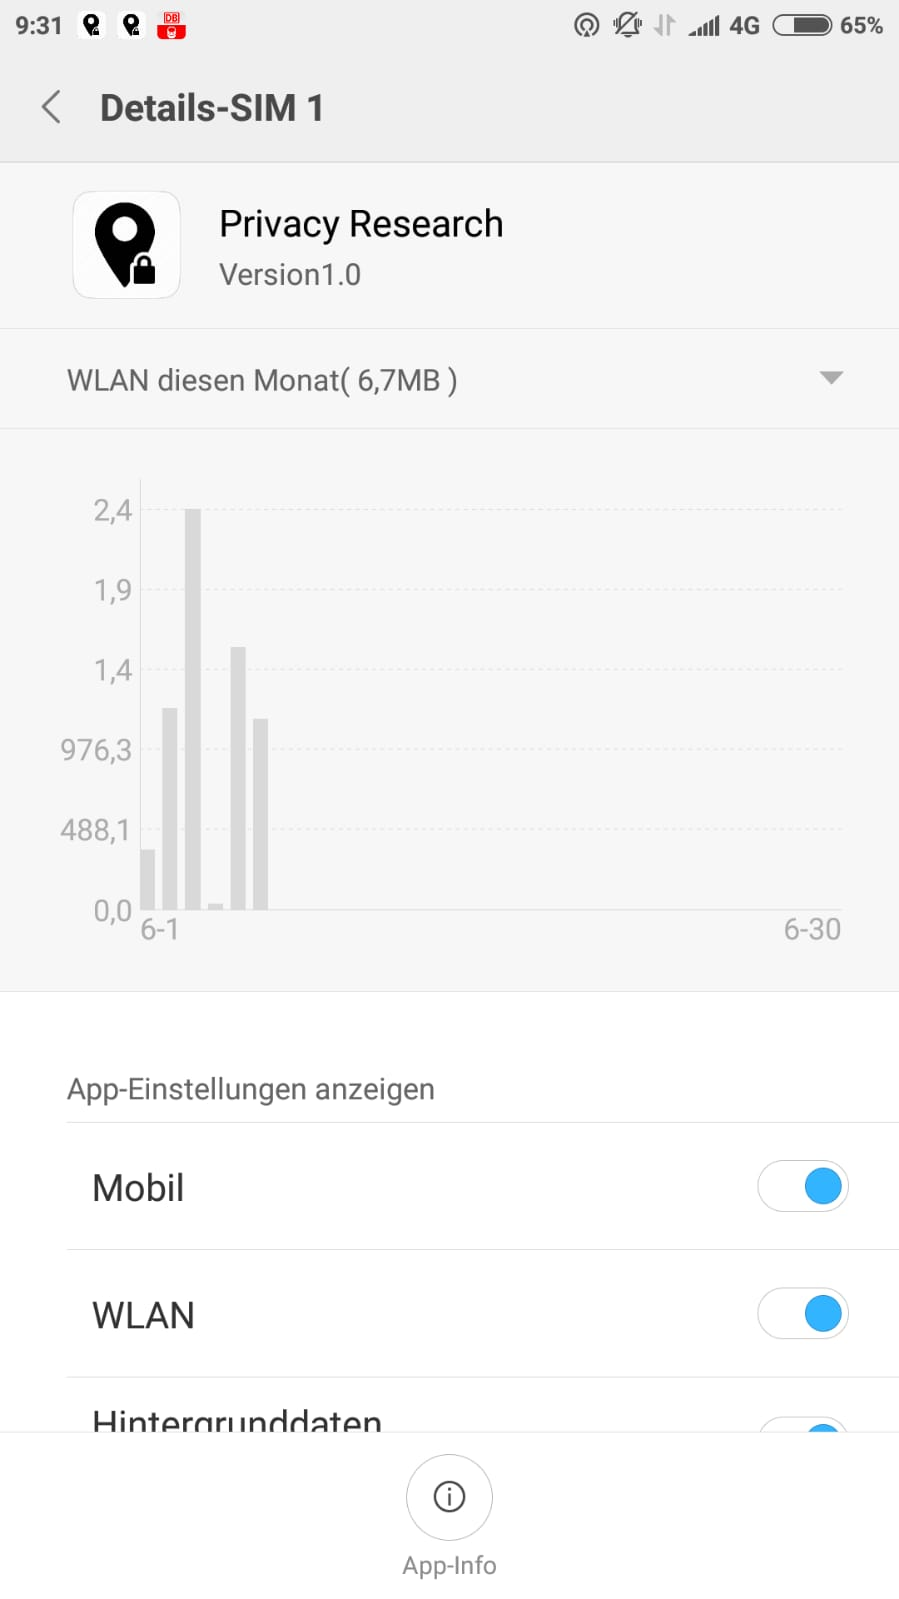
\includegraphics[width=200pt]{data/data-usage/data-usage2-1.jpeg}
\end{center}
\begin{center}
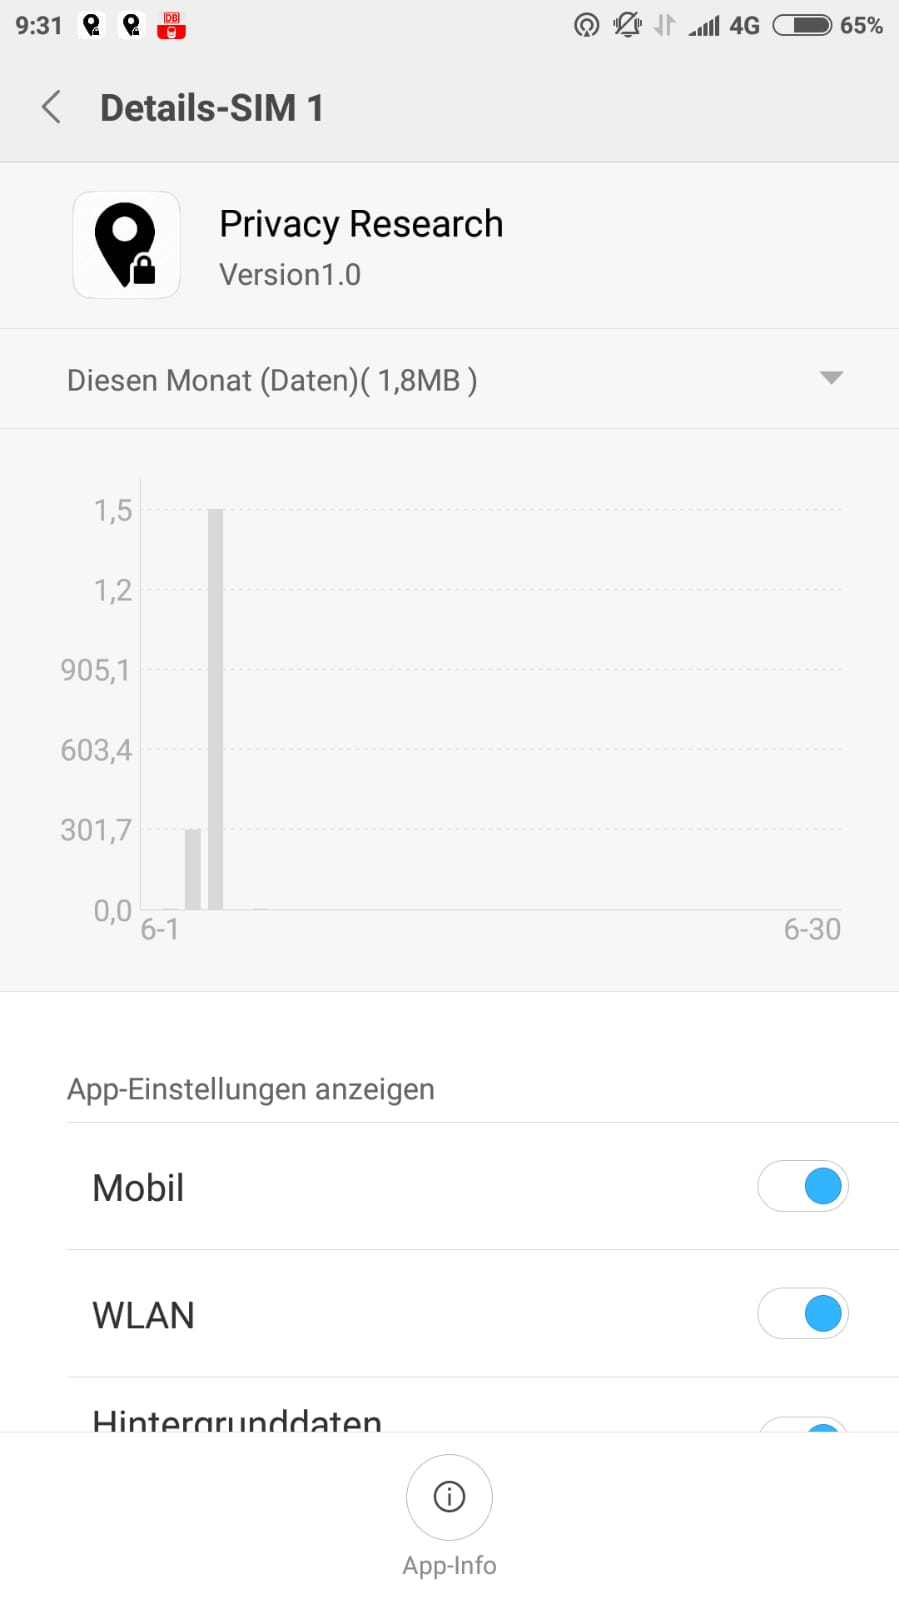
\includegraphics[width=200pt]{data/data-usage/data-usage2-2.jpeg}
\end{center}
\begin{center}
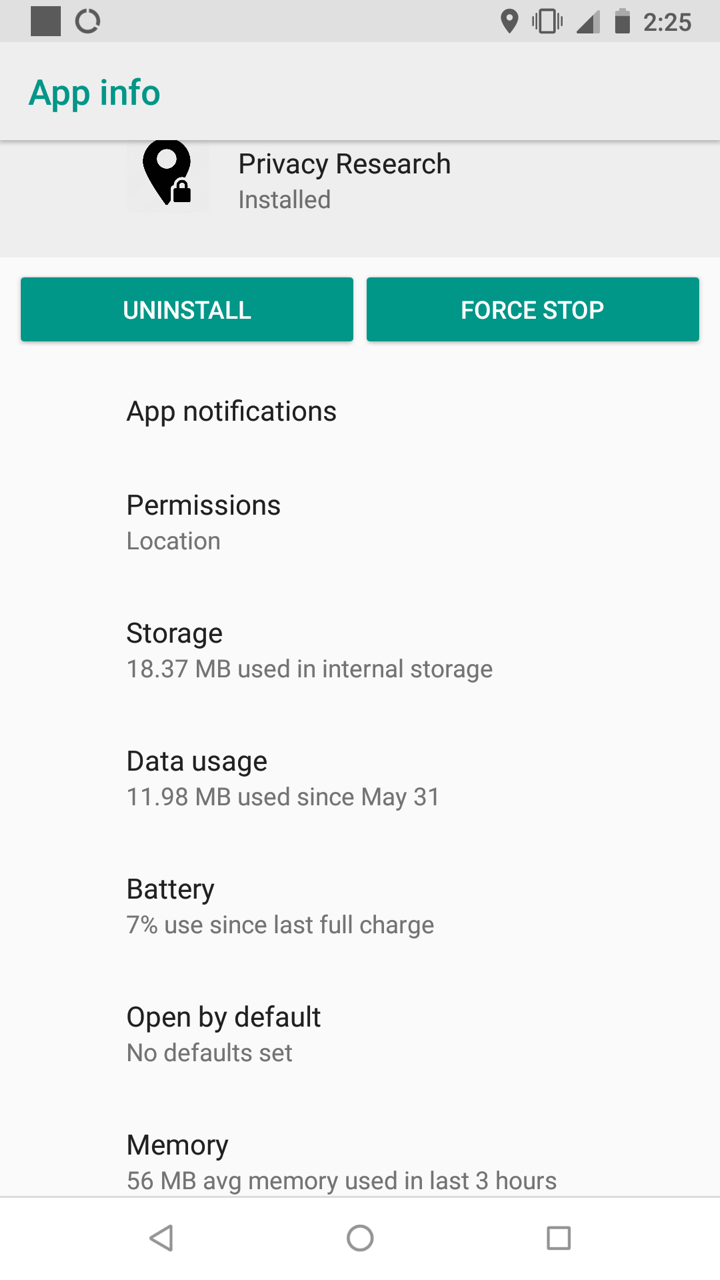
\includegraphics[width=200pt]{data/data-usage/data-usage3.png}
\end{center}
\begin{center}
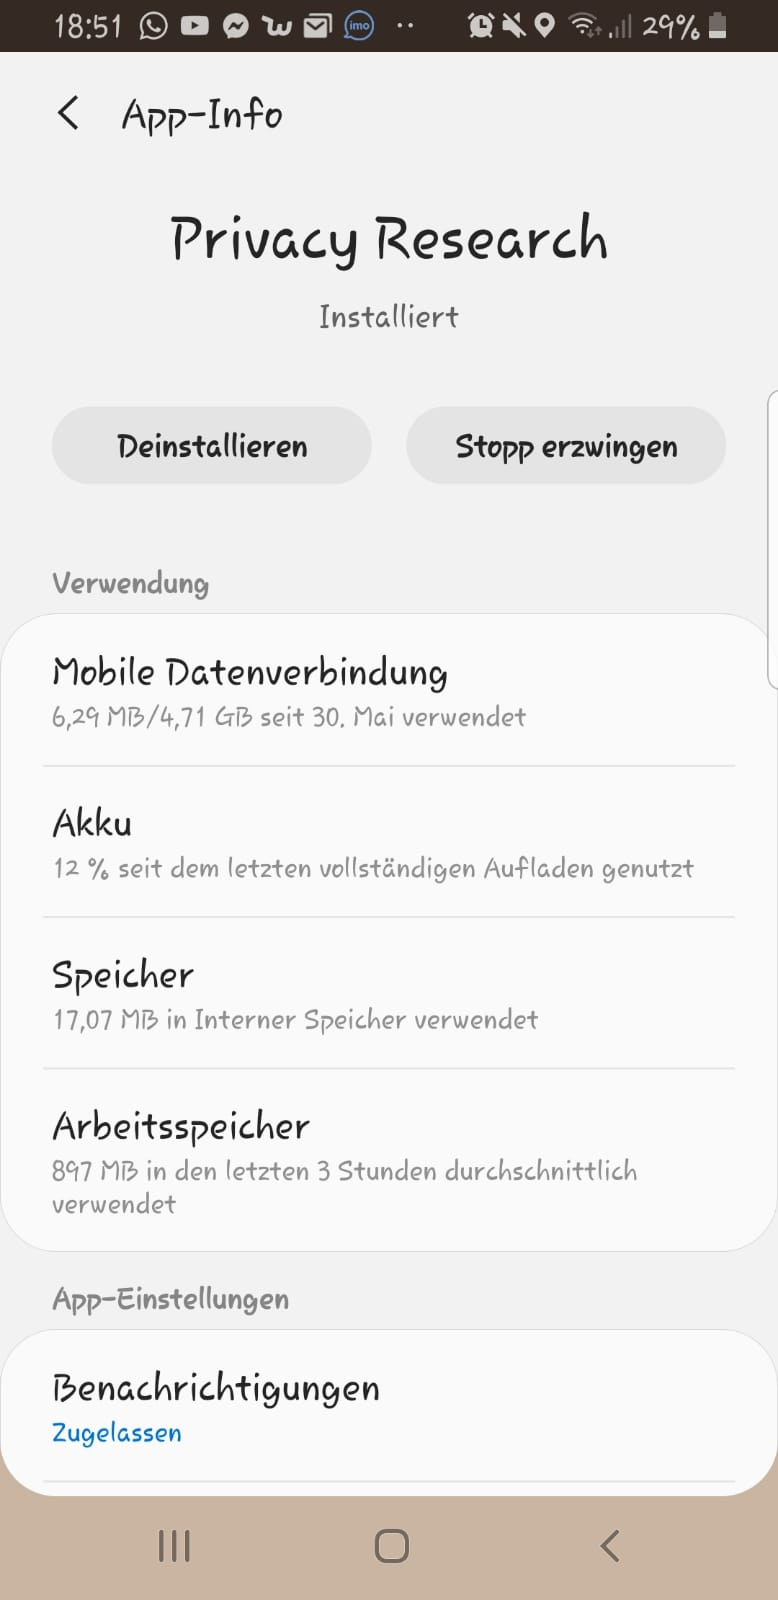
\includegraphics[width=200pt]{data/data-usage/data-usage4.jpeg}
\end{center}
\begin{center}
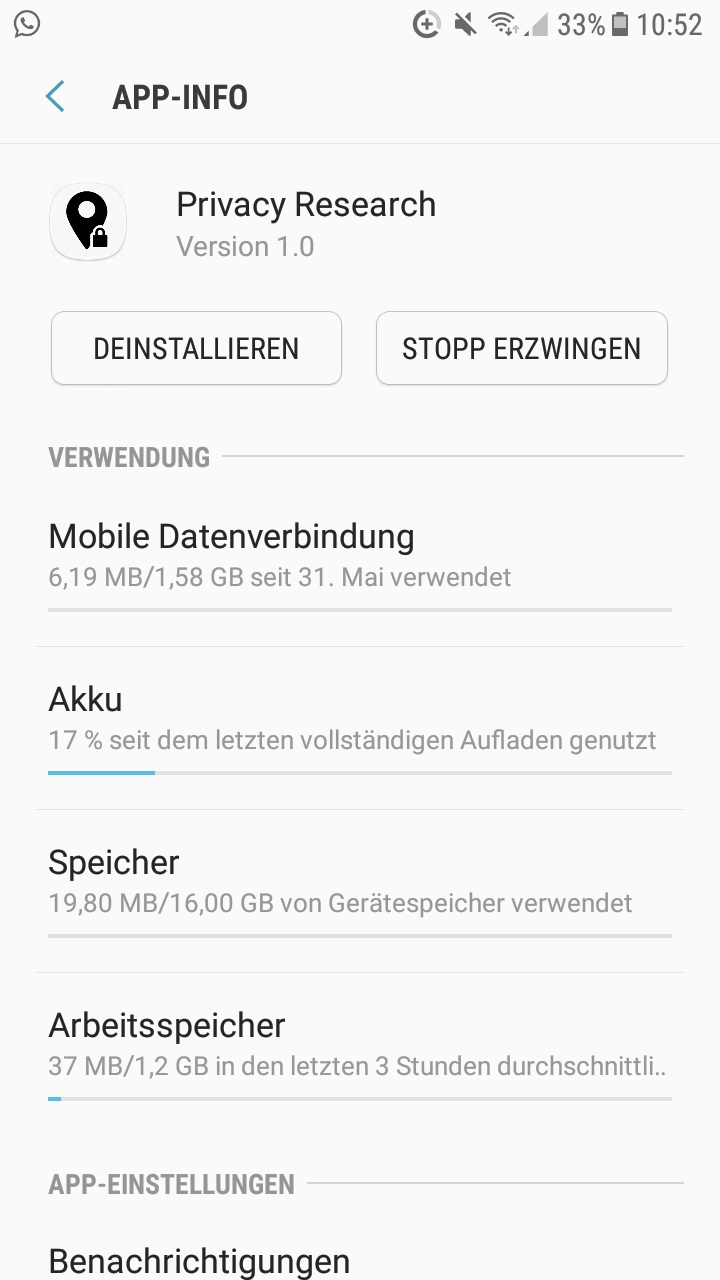
\includegraphics[width=200pt]{data/data-usage/data-usage5.jpeg}
\end{center}
\begin{center}
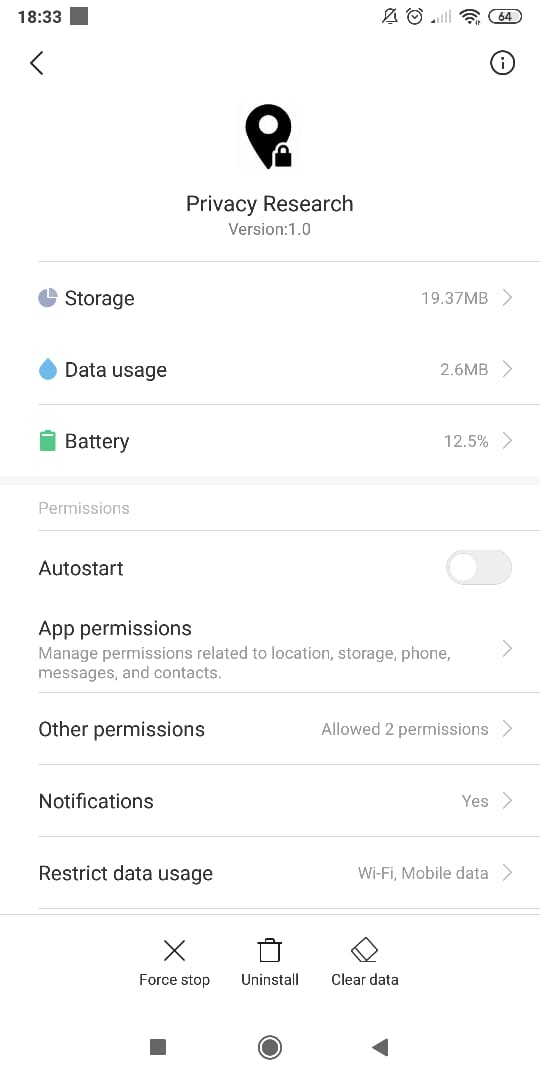
\includegraphics[width=200pt]{data/data-usage/data-usage6.jpeg}
\end{center}
\begin{center}
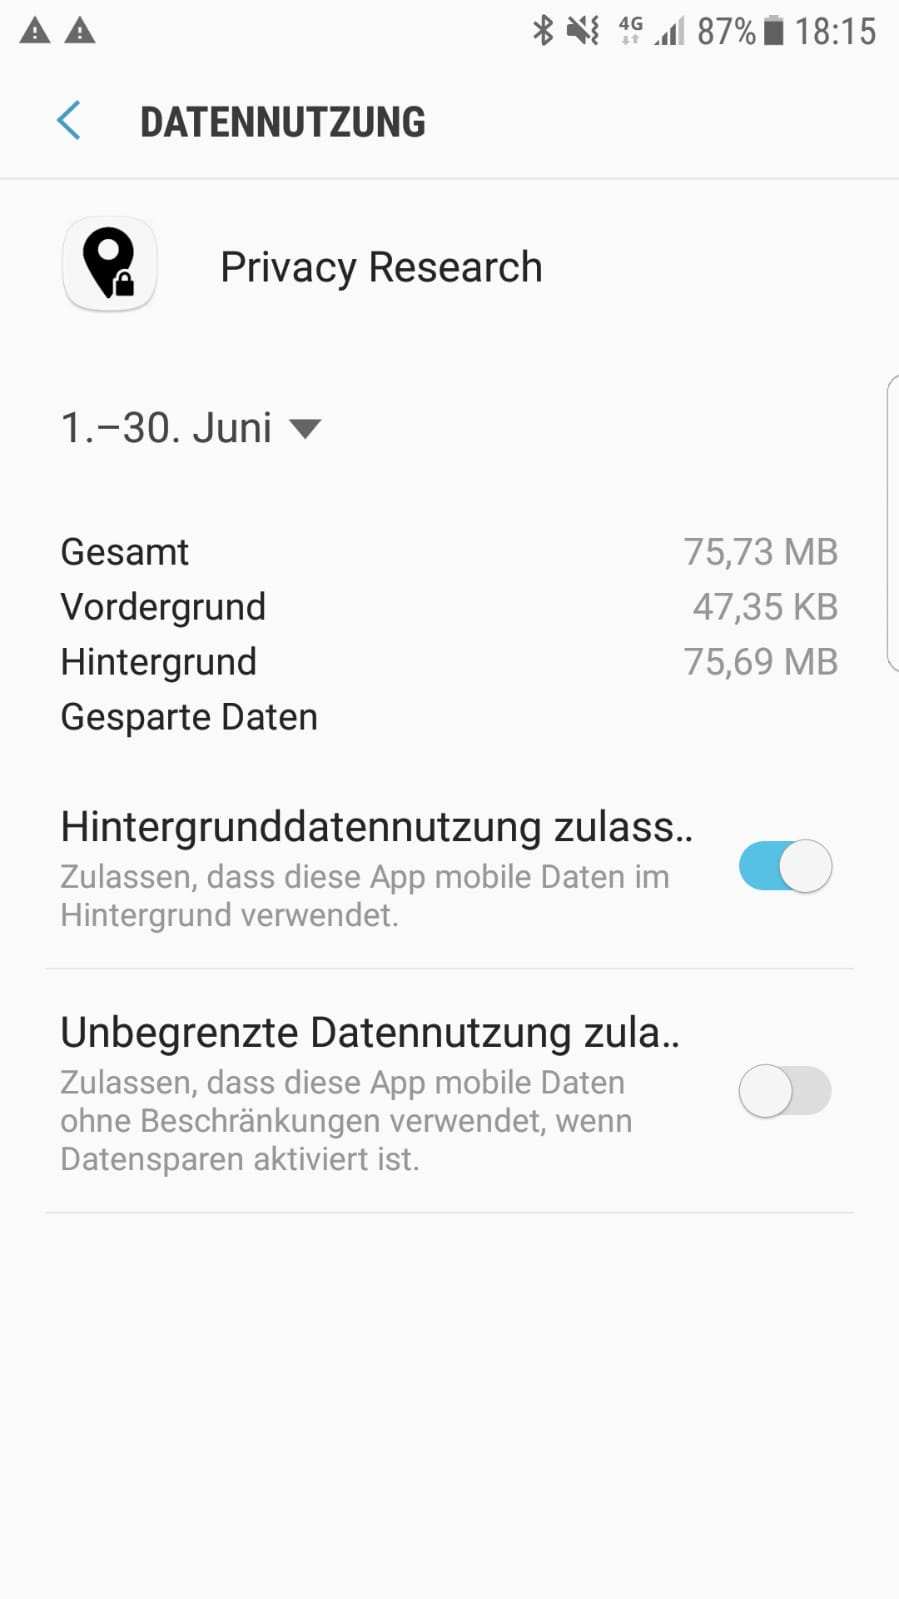
\includegraphics[width=200pt]{data/data-usage/data-usage7.jpeg}
\end{center}
\begin{center}
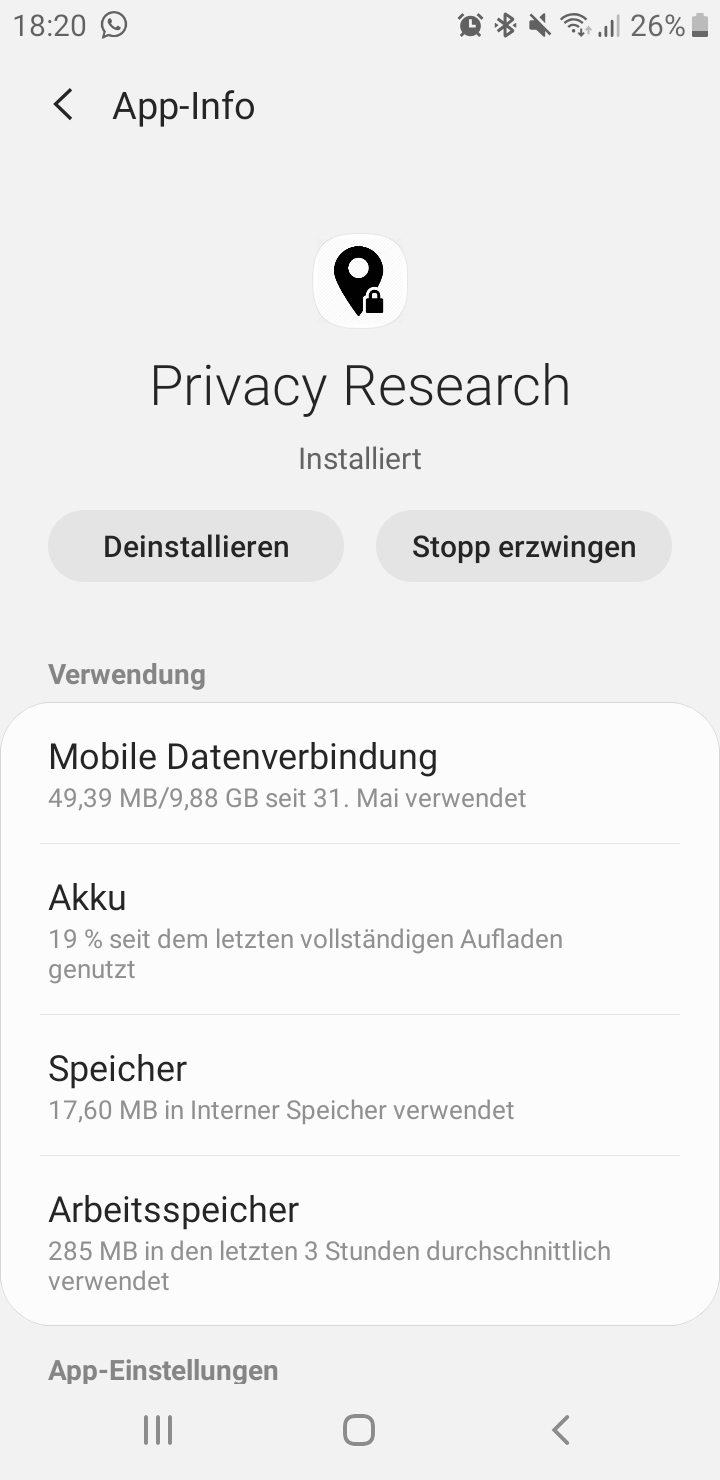
\includegraphics[width=200pt]{data/data-usage/data-usage8.jpeg}
\end{center}
\begin{center}
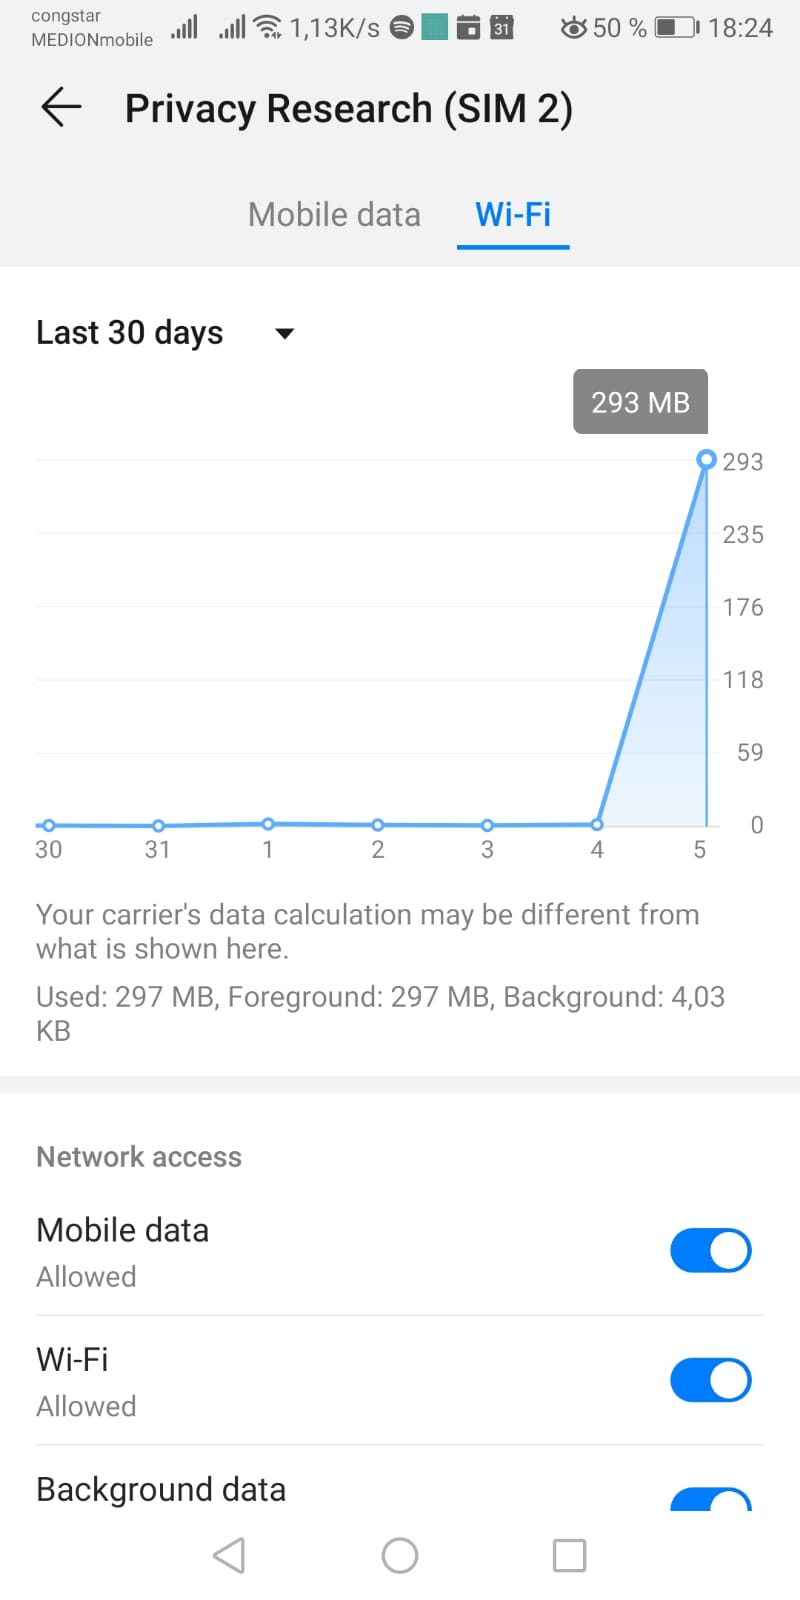
\includegraphics[width=200pt]{data/data-usage/data-usage9-1.jpeg}
\end{center}
\begin{center}
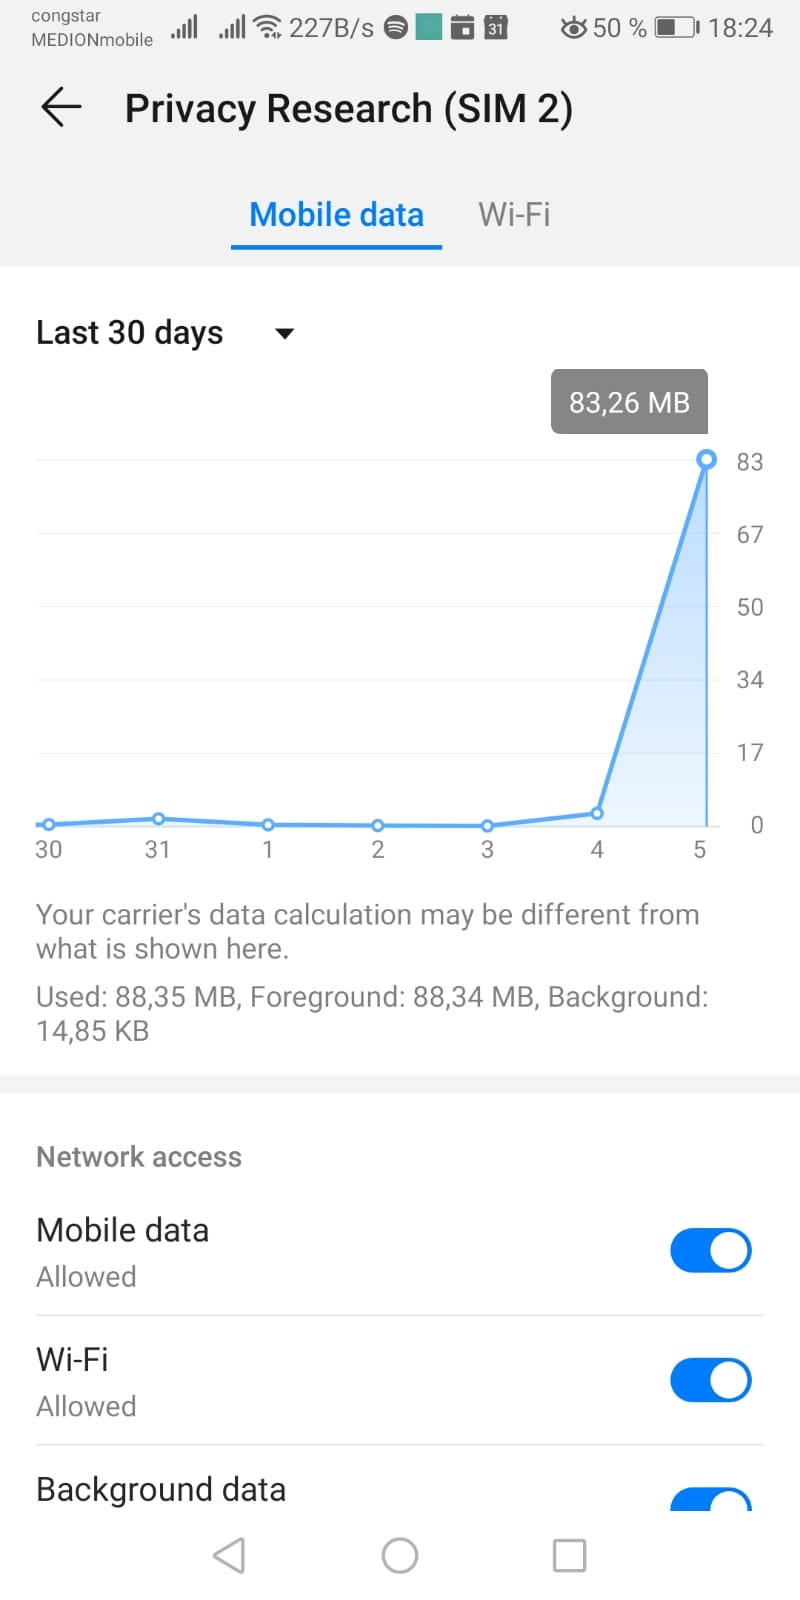
\includegraphics[width=200pt]{data/data-usage/data-usage9-2.jpeg}
\end{center}